\documentclass{beamer}
\usetheme{Darmstadt}
\usepackage{CJKutf8}

\usepackage[utf8]{inputenc}
\usepackage[OT1, T2A]{fontenc}
\usepackage{fontspec}
\usepackage[normalem]{ulem}

\usepackage{graphicx}
\usepackage{tikz}
\usepackage{braket}

\usepackage{xcolor}
\usepackage{pgfplots}
\usepackage{tikz}

\begin{document}
    \begin{frame}{S-DES}
        \begin{itemize}
            \item Simplified DES with 2 rounds
            \item Structure similar to DES but simplified with 10-bit key and 8-bit plaintext.
            \item Quantum oracle needs to be reversible, of which S-DES is (normally) not.
        \end{itemize}
    \end{frame}

    \begin{frame}{Structure of S-DES}
        \begin{figure}[h]
            \centering
            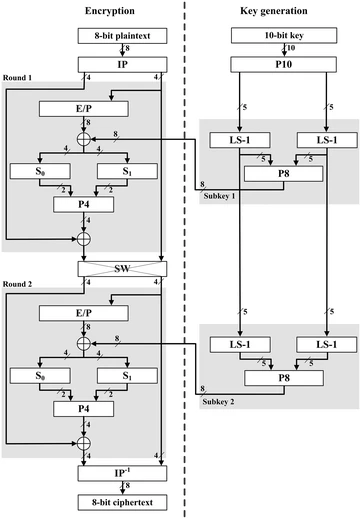
\includegraphics[width=0.5\textwidth]{./Images/sdes.png}
        \end{figure}
    \end{frame}

    \begin{frame}{Structure of S-DES}
        Consists of two main parts:
        \begin{itemize}
            \item Key Scheduling, where we generate subkeys from the given key
            \item Feistel function, where we encrypt the plaintext using the scheduled keys
        \end{itemize}
    \end{frame}

    \begin{frame}{Structure of S-DES: Key Scheduling}
        \begin{figure}[h]
            \centering
            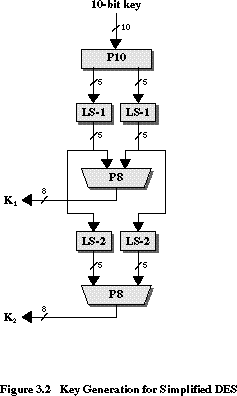
\includegraphics[width=0.5\textwidth]{./Images/keygen.png}
        \end{figure}
    \end{frame}

    \begin{frame}{Structure of S-DES: Feistel function}
        \begin{figure}[h]
            \centering
            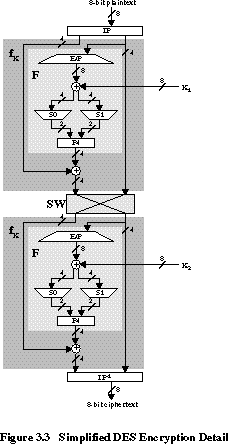
\includegraphics[width=0.38\textwidth]{./Images/feistel.png}
        \end{figure}
    \end{frame}

    \section{Grover's Algorithm}

    \begin{frame}{Overview}
        \begin{itemize}
            \item Grover's algorithm can find a specific state satisfying some condition among $ N = 2^n$ candidates in $ O(\sqrt{N}) $ time, compared to classical runtime complexity $ O(N) $.
            \item Grover's algorithm exploits qualities of quantum amplitudes to gain advantage of probability seperation.
            \item It can brute-force 128-bit symmetric cryptographic key in roughly $ 2^{64} $ iterations.
        \end{itemize}
    \end{frame}

    \begin{frame}{Algorithm}
        Input:
        \begin{itemize}
            \item A quantum oracle $ \mathcal{O} $ which performs the operation $ \mathcal{O} \ket{x}  = (-1)^{f(x)} \ket{x}$, where $ f(x) = 0 $ for all $0 \leq x < 2^n $ except $ x_0 $, for which $ f(x_0) = 1 $.
            \begin{itemize}
                \item Such quantum oracle is viable, and takes $ O(1) $ time.
            \end{itemize}
            \item $ n $ qubits initialized to the state $ \ket{0} $
        \end{itemize}
        Output: $ x_0 $, in runtime $ O(\sqrt{2^n}) $ with error rate $ O(\frac{1}{2^n}) $
    \end{frame}

    \begin{frame}{Algorithm}
        Procedure:
        \begin{enumerate}
            \item $ \ket{0}^{\otimes n} $ (initial state)
            \item $ H^{\otimes n} \ket{0}^{\otimes n} = \dfrac{1}{\sqrt{2^n}} \sum\limits_{x=0}^{2^n-1}\ket{x} = \ket{\psi}$ (Hadamard transform)
            \item $ [(2 \ket{\psi} \bra{\psi} - I) \mathcal{O}]^R \ket{\psi} \approx \ket{x_0}  $ (Grover iteration for $ R \approx  \frac{\pi}{4}\sqrt{2^n} $ times)
            \item $ x_0 $ (measure)
        \end{enumerate}
        Grover iteration in a nutshell: negate the amplitude of the desired state, followed by `diffusion transform' which increases the amplitude of the desired state and lower the others.
    \end{frame}
\end{document}